\documentclass[11pt]{beamer}
% \usetheme{Copenhagen}
\usetheme{PaloAlto}
\usepackage[utf8]{inputenc}
\usepackage[spanish]{babel}
\usepackage{amsmath}
\usepackage{amsfonts}
\usepackage{amssymb}
\usepackage{graphicx}
\graphicspath{{figures/}}
\usepackage{ragged2e}
\usepackage{xcolor}
\usepackage{hyperref}
\hypersetup{urlcolor=blue}
\author{Carlos Espinosa}
\title{Software y SOs}
%\setbeamercovered{transparent} 
%\setbeamertemplate{navigation symbols}{} 
\logo{
\includegraphics[width=1.4cm]{fac-logo-w}} 
\institute{Facultad de Ciencias \\ Universidad Nacional Autónoma de México} 
\date{Septiembre, 2022} 
% \subject{} 

\justifying
\begin{document}
\begin{frame}
\titlepage
\end{frame}

%\begin{frame}
%\tableofcontents
%\end{frame}
\section{Introducción}
	\subsection{Software}
		\begin{frame}{Software de una computadora}
			Para nuestros propósitos, software es una palabra que significa programas.
			
			Un programa es una específica, precisa y detallada descripción de:
			\begin{itemize}
				\item una colección de datos, en RAM, disco, etc.
				\item una secuencia de acciones de esos datos
			\end{itemize}
			
			Las acciones en un programa son conocidos como instrucciones.
			
			En computación, los datos son valores almacenados en lugares de almacenamiento, como RAM, disco, etc
		\end{frame}
		\begin{frame}{Que son las instrucciones?}
			Las acciones en un programa son conocidas como instrucciones.
			
			\begin{itemize}
				\item Cálculos aritméticos/logicos
				\item Operaciones de memoria: cargar o guardar en RAM
				\item I/O: leer de o escribir a almacenamiento secundario.
				\item Ejecutar instrucciones en cierta secuencia.
				\item Repetición
			\end{itemize}
			...etc.
		\end{frame}
	\subsection{Sistema operativo}
		\begin{frame}{Sistema operativo}
			Un sistema operativo es un programa que controla la ejecución de todos los otros programas. Esto lo hace el programa más importante en una computadora.
			 \begin{columns}
			 	\begin{column}{0.5\textwidth}
					El SO (OS) actua como una interface entre la computadora y el usuario. Es responsable de la administración y coordinación de las actividades y la repartición de los recursos de la computadora
				\end{column}
				\begin{column}{0.5\textwidth}
					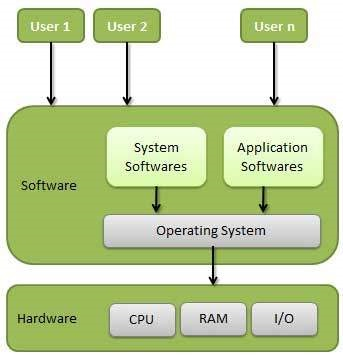
\includegraphics[scale=0.5]{so.jpg}
				\end{column}
			\end{columns}
		\end{frame}
		\begin{frame}{Sistema operativo: responsabilidades}
			\begin{itemize}
				\item Tareas básicas: reconocer la entrada del teclado, enviar información de salida a la pantalla, mantener la ubicación de los archivos y directorios en el disco y controlar los dispositivos periféricos como discos extraibles e impresoras.
				\item Asegurarse que los diferentes programas y los usuarios que corren al mismo tiempo no interfieran unos con otros.
				\item Proveer una plataforma de software sobre el cual otros programas puedan correr.
			\end{itemize}
			Los SO también son responsables sobre la seguridad y asegurarse que los usuarios sin autorización no accesan al sistema.
		\end{frame}
		\begin{frame}{Sistema operativo: responsabilidades}
			Tareas mayores
			\begin{itemize}
				\item Manejo de recursos
				\begin{itemize}
					\item Asigna los recursos de la computadora tal como el tiempo de CPU, la memoria principal, el uso de dispositivos de entrada y salida.
				\end{itemize}
				\item Manejo de información
				\begin{itemize}
					\item Gobierna la entrada y salida de información y su ubicación, almacenamiento y recuperación.
					\item Es responsable del almacenaje y recuperación de información en discos. También se encarga de la organización de la información en este medio.
				\end{itemize}
			\end{itemize}
		\end{frame}
		\begin{frame}{Sistema operativo: responsabilidades}
			Tareas mayores
			\begin{itemize}				
				\item Manejo de trabajos
				\begin{itemize}
					\item Prepara, agenda, controla y monitoriza los trabajos mandados a ejecutarse para asegurar un procesamiento eficiente.
					\item Un trabajo es una colección de uno o mas programas relacionados y su información.
				\end{itemize}
				\item Establece el estándar de la comunicación entre el usuario y la computadora.
				\begin{itemize}
					\item Se establece un estandar de comunicación entre los usuarios y sus sistemas computacionales.
					\item Lo hace al proveer una interfaz de usuario y un  conjunto de comandos estandar que controlan el hardware.
				\end{itemize}
			\end{itemize}
		\end{frame}
		\begin{frame}{Sistema operativo: Interfaz de usuario}
			\begin{itemize}
				\item Es un programa que controla un monitor para el usuario y permite que el usuario interactue con el sistema.
				\item La interfaz de usuario permite al usuario comunicarse con el SO
				\item La interfaz de usuario provee el significado de:
				\begin{itemize}
					\item Entrada: Permite a los usuarios manipular el sistema
					\item Salida: Permita al sistema indicar los efectos de la manipulación del usuario.
				\end{itemize}
				\item Hay dos tipos de interfaz
				\begin{itemize}
					\item Interfaz de línea de comandos
					\item Interfaz de usuario gráfico
				\end{itemize}
			\end{itemize}
		\end{frame}
	\subsection{Tipos de SOs}
		\begin{frame}{Tipos de sistemas operativos}
			Podemos distinguir distintos tipos de SO por sus características:
			\begin{itemize}
				\item En tiempo real (Real-time)
				\item Multi usuario vs Mono usuario
				\item Multi tarea vs Mono Tarea
				\item Distribuido
				\item Incrustados
			\end{itemize}
		\end{frame}
		\begin{frame}{Tipos de sistema operativos}
			En tiempo real:
			\begin{itemize}
				\item Un SO en tiempo real es un SO multitarea que se enfoca en ejecutar en tiempo real las aplicaciones
				\item Responde a la información de entrada instantáneamente.
			\end{itemize}
			Multi usuario vs Mono usuario:
			\begin{itemize}
				\item Un SO multi usuario permite a multiples usuarios accesar a una computadora al mismo tiempo.
				\item Un sistema de tiempo compartido puede ser clasificado como un sistema multi usuario dado que permiten el acceso a multiples usuarios a través de compartir el tiempo.
				\item Sistemas mono usuario solo pueden ser usados por un usuario a la vez.
			\end{itemize}
		\end{frame}
		\begin{frame}{Tipos de sistemas operativos}
			Multi tarea vs mono tarea
			\begin{itemize}
				\scriptsize
				\item Un SO es mono tarea si solo permite correr un programa al a vez.
				\item Un SO multi tarea permite la ejecución de multiples tareas al mismo tiempo.
			\end{itemize}
			Distribuido
			\begin{itemize}
				\scriptsize
				\item Un SO distribuido administra un grupo computadoras independientes y las hace parecer una sola computadora.
				\item El desarrollo de las computadoras en red permitió que pudieran conectarse y comunicarse unas con otros, dando origen a computo distribuido.
			\end{itemize}
			Incrustado
			\begin{itemize}
				\scriptsize
				\item Los SO incrustados están diseñados para ser usados en sistemas de computo incrustados (Disp. con una tarea especifica: microondas, bombas de gasolina, control de crucero, sistemas intelgentes, etc.).
				\item Están diseñados para operar en pequeñas máquinas como PDA's con menos autonomía.
				\item Son capaces de operar con un número limitado de recursos.
			\end{itemize}
		\end{frame}
\section{Windows}
	\subsection{MS-DOS}
		\begin{frame}{MS-DOS y Windows}
			Windows es un sistema operativo que estaba basado en MS-DOS.
			
			\begin{itemize}
				\item Las primeras versiones del sistema operativo, llamado QDOS, fueron lanzadas en agosto de 1980. QDOS significaba \textit{Quick and Dirty Operating System}.
				\item Se desarrollo de manera rápida pero trabajaba sorprendentemente bien. Tenía las herramientas necesarias para un desarrollo de lenguaje ensamblador pero sin editor.
				\item Una semana después, se creo con un editor, EDLIN (editor of lines)
			\end{itemize}
		\end{frame}
		\begin{frame}{MS-DOS y Windows}
			\begin{itemize}
				\item Además de QDOS, existía otra variante de DOS como 86-DOS. Microsoft compró los derechos en 1981 de \textit{Seattle Computer} y lo llamó MS-DOS, \textit{Microsoft's Disk Operating System}
				\item MS-DOS fue el primer SO a grande escala comercialmente hablando. Fue el primero en ser un SO de propósito general ya que corría en múltiples configuraciones de hardware.
				\item IBM por su parte desarrollaba PC-DOS (Personal Computer Disk Operating System) el cual estaba basado en QDOS, el cual fue licenciado por Microsoft.
			\end{itemize}
			Después de lanzar la versión 1.25 y 2.0 de MS-DOS en 1982 y 1983, respectivamente. En 1983, Microsoft anuncia que desarrollarán una versión gráfica de MS-DOS.
		\end{frame}
	\subsection{Estructura de MS-DOS}
		\begin{frame}{MS-DOS y Windows}
			Estructura de MS-DOS
			\begin{itemize}
				\item Basic Input/Output System (BIOS): Específico de cada sistema y es provisto por el fabricante del hardware. Contiene controladores para el hardware básico: el monitor, teclado, servicio de booteo, etc. este es provisto por el fabricante de hardware.
				
				Los componentes más primitivos del BIOS, llamados porción recidente, es guardado en ROM y cargado a RAM cuando el sistema se inicia.
				
				El kernel se comunica con el dispositivo mediante paquetes de solicitudes I/O.  Estas solicitudes son traducidas a una forma correcta de comando a los distintos componentes de hardware por los controladores.
			\end{itemize}
		\end{frame}
		\begin{frame}{MS-DOS y Windows}
			Estructura de MS-DOS
			\begin{columns}
				\begin{column}{0.5\textwidth}
					\scriptsize
					\begin{itemize}
						\item El kernel de DOS es el intermediario entre los servicios obligatorios del SO y las funciones que son independientes del hardware. Estas funciones son administración de archivos y memoria, control de dispositivos de I/O, invocar otros programas, accesar al reloj de tiempo real, etc.
						\item El kernel de MS-DOS es muy parecido en cada sistema, sin importar el fabricante. El Kernel es cuardado en el disco en un archivo llamado MSDOS.SYS el cual está oculto.
					\end{itemize}
				\end{column}
				\begin{column}{0.5\textwidth}
					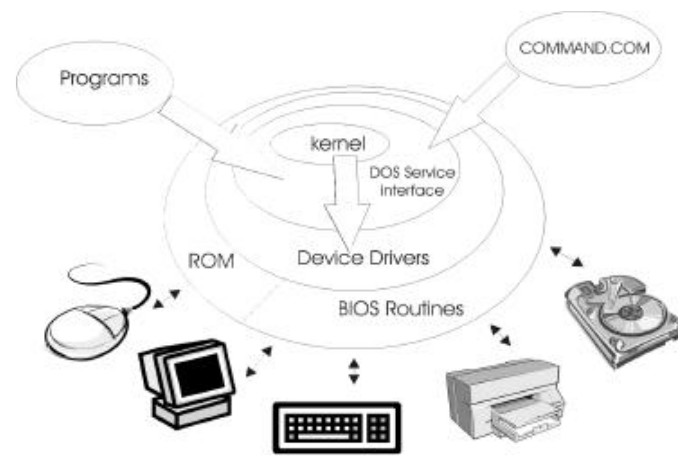
\includegraphics[scale=0.3]{kernel.jpg}
				\end{column}
			\end{columns}
		\end{frame}
		\begin{frame}{MS-DOS y Windows}
			Estructura de MS-DOS
			\begin{itemize}
				\item El procesador de comandos provee la interfaz de usuario de MS-DOS. Este muestra una línea de comandos donde el usuario escribirá comandos y los ejecutará.
				\item El procesador de comandos será el responsable de proveer rastrear errores y proveer la respuesta a ellos. El kernel es requerido y no puede ser modificado, el procesador de comando no es requerido.
				\item El procesador de comandos puede ser desarrollado por quien sea, algunos vendedores pueden no implementarlo.
			\end{itemize}
		\end{frame}		
	\subsection{Historia de Windows}
		\begin{frame}{Historia de Windows}
			A finales de 1983, Microsoft anuncia Windows 1.0. A pesar de estp, aún lanzaría al mercado MS-DOS 2.11, MS-DOS 2.25, MS-DOS 3.0 y MS-DOS 3.1 entre 1983 y 1984.
			
			A finales de 1985, la primera versión de Windows fue introducida al mercado.
			
			\textbf{Windows 1.0}
			\begin{itemize}
				\item Esta versión tenía como principal concepto de hacerlo multitarea y hacerlo gráfico.
				\item Introdujo por primera vez las ventanas en una primera versión.
				\item Tenía reloj, calendario, portapapeles, cartas de archivo, panel de control, editor note pad, Paint, utilerías de escritura y Reversi
			\end{itemize}
			Estaba provisto de un intérpetre de comandos (shell) llamado MS-DOS EXECTIVE
		\end{frame}
		\begin{frame}{Historia de Windows}
			Una imagen de como era Windows 1.0
			
			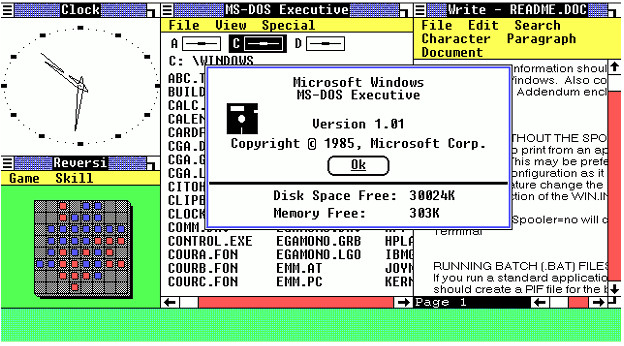
\includegraphics[scale=0.7]{w1.jpg}
		\end{frame}
		\begin{frame}{Historia de Windows}
			A finales de 1987 salió Windows 2.0 y 2.1.X. También salieron las versiones Windows/286 y Windows/386.
			
			\begin{itemize}
				\item Esta versión permitia que las ventanas se sobrepusieran.
				\item La multitarea, el uso del mouse y el bitmap fueron introducidos así como un mejor entorno gráfico.
				\item En esta versión se empezaron a usar las palabras minimizar y maximizar (Zoom e iconizar anteriormente)
				\item Se incluia Notepad, calendario, reloj, terminal, Reverse 1, Paint, portapapeles, calculadora, etc.
			\end{itemize}
			Apple demandó a Microsoft por violación de derechos de autor dado que las interfaz de ambos eran muy parecidas.
		\end{frame}
		\begin{frame}{Historia de Windows}
			Una imagen de como era Windows 2.0
			
			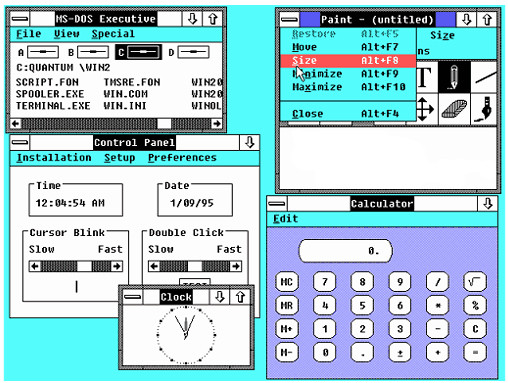
\includegraphics[scale=0.6]{w2.jpg}
		\end{frame}
		\begin{frame}{Historia de Windows}
			\small
			En el año de 1990 salió Windows 3.0 (MS-DOS seguía en desarrollo. Para cuando salió Windows 3.0, MS-DOS ya estaba en su versión MS-DOS 4.01a). Esta versión de Windows mejoro el ambiente del usuario al igual que el ambiente técnico que usaba mejor las capacidades de emoria de los procesador 80286 y 80386.
			\begin{itemize}
				\item Se mejoró la multitarea, se introdujo administrador de programas y administrador de archivos que reemplazaron al DOS executive.
				\item Se siguió usando el sistema de colores de 16-bit. Se agregaron diferentes estilos de fuente y se incluyeron tres diferentes modos de memoria.
				\item Se implementó la memoria virtual
				\item Se incluyó un soporte para archivos multimedia, de audio.
				\item Fue la primera versión en ser preinstalada en discos duros.
				\item Se introdujo el buscaminas e IE 2.0, reproductor de archivos multimedia e integración para CD-ROM
			\end{itemize}
		\end{frame}
		\begin{frame}{Historia de Windows}
			Una imagen de como era Windows 3.0
			
			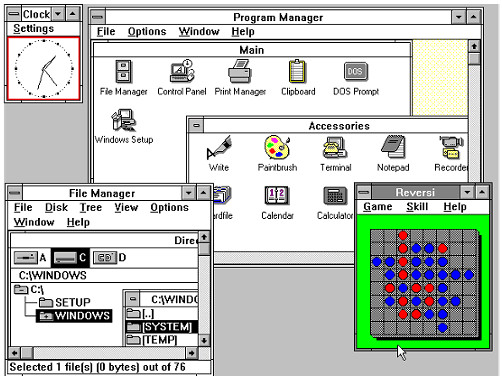
\includegraphics[scale=0.6]{w3.jpg}
		\end{frame}
		\begin{frame}{Historia de Windows}
			\small
			A partir de este punto, se adoptó una nueva terminología basado en 9x.
			
			En agosto de 1995 salió a la venta Windows 95 la cual estaba separada de las versiones MS-DOS de Windows, aunque aun muy en el fondo aún ejecutaba MS-DOS. Tenía una gran cantidad de controladores de dispositivos virtuales que eran los reponsables de administrar los dispositivos como el monitor, video, tarjetas de red, etc.
			
			Algunos de estos controladores virtuales eran:
			\begin{itemize}
				\item	Máquina virtual: era el kernel y se encargaba de administrar la memoria, eventos, tratar con las interrupciones, administraba los controladores y agendaba las tareas.
				\item Administrador de configuraciones: revisa el estado de todos los dispositivos unidos a la computadora y funcionaba como el controlador de las modificaciones de estado, si estaban activos, etc.
				\item Administrador del sistema de archivos: definia el sistema de acceso a varios archivos. Se encargaba de la barra de inicio, barra de tareas, del explorador de archivos, etc.
			\end{itemize}
		\end{frame}
		\begin{frame}{Historia de Windows}
			Una imagen de como era Windows 95
			
			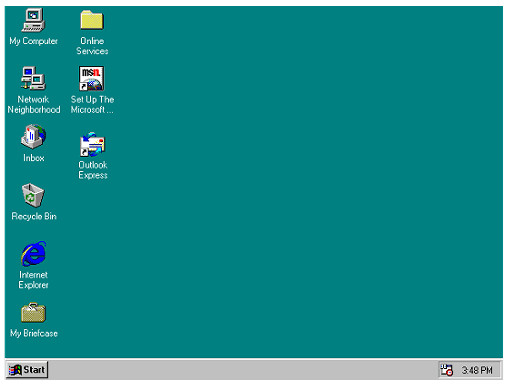
\includegraphics[scale=0.6]{w95.jpg}
		\end{frame}
		\begin{frame}{Historia de Windows}
			En Junio de 1998 fue lanzado al mercado Windows 98. Esta versión soportaba 32 bits.
			
			\begin{itemize}
				\item En esta edición se introdujo el Windows Driver Model (WDM). Esta nueva tecnología facilita el desarrollo de controladores para dispositivos.
				\item En esta versión se incluyeron el Scan Disk, Disk Defragmenter, Scan Reg, MS config.
				\item Se mejoró el soporte del sistema a el Universal Serial Bus
				\item Fue introducida la Local Area network con lo que podría comunicarse con otros sistemas.
				\item Se dió soporte a DVD-ROM
			\end{itemize}
		\end{frame}
		\begin{frame}{Historia de Windows}
			Una imagen de como era Windows 98
			
			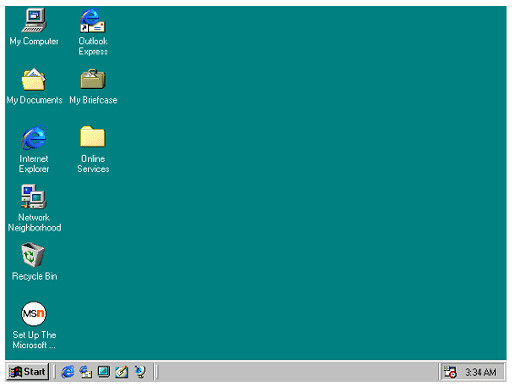
\includegraphics[scale=0.6]{w98.jpg}
		\end{frame}
		\begin{frame}{Historia de Windows}
			Windows 2000 fue lanzado a inicios del año 2000. Esta versión tuvo cuato ediciones: Professional, Server, Advanced Server y Data centre Server
			\begin{itemize}
				\item Se uso el sistema de archivos FAT32 y fue introducido el NTFS 3.0
				\item Se incluyeron características para servidores
				\item Se ampliaron las aplicaciones de administración
				\item Se agrego soporte para dispositivos de almacenamiento masicos (Controladores USB)
				\item IE 5.0, Outlook express y se habilitó la compartición de conexión a internet 
				\item Sistema avanzado de recovery, sistema de archivos encriptados y protección extendida de información
			\end{itemize}
		\end{frame}
		\begin{frame}{Historia de Windows}
			Una imagen de como era Windows 2000
			
			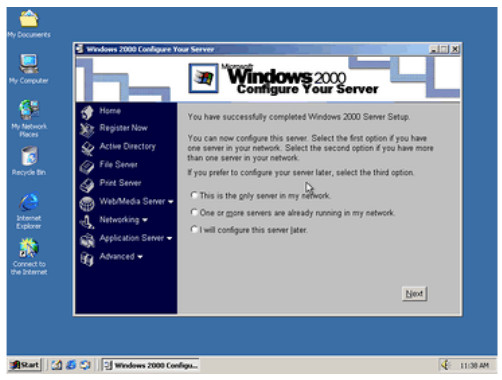
\includegraphics[scale=0.6]{w2k.jpg}
		\end{frame}
		\begin{frame}{Historia de Windows}
			Windows Me fue lanzado en septiembre de 2000. Esta versión fue hecha para computadores en hogares.
			\begin{itemize}
				\item IE 5.5
				\item Windows Movie Maker y Windows Media Player 7
				\item Se habilitó DirectX
				\item Dial up networking, TCP/IP, Home nertworking wizards, etc.
				\item Herramientas del sistema: Administrador de sistema, sistema de protección de archivos.
			\end{itemize}
		\end{frame}
		\begin{frame}{Historia de Windows}
			Una imagen de como era Windows Me
			
			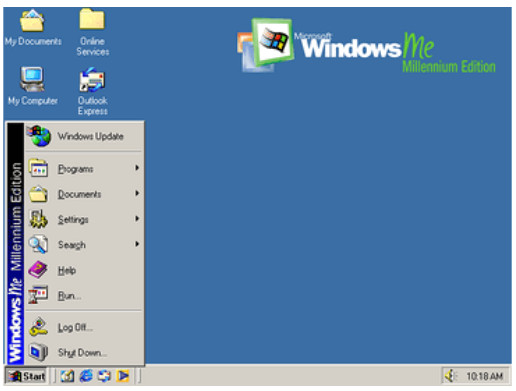
\includegraphics[scale=0.6]{wme.jpg}
		\end{frame}
		\begin{frame}{Historia de Windows}
			La arquitectura básica del SO cambio de un kernel basado en MS-DOS a un kernel basado en NT.
			Windows XP fue lanzado en octubre de 2001. Soportaba una arquitectura de 32 bits y de 64 bits.
			
			Algunas de las características nuevas fueron:
			\begin{itemize}
				\item Barra de tareas y menu de inició
				\item Windows explorer
				\item Estructura de gráficos mejoradas
				\item Mejoras de estructura
				\begin{itemize}
					\item Inicio rápido y de inicio de sesión
					\item Opción de busqueda
					\item Plug and Play
					\item Temas de escritorio
				\end{itemize}				
			\end{itemize}
		\end{frame}
		\begin{frame}{Historia de Windows}
			Una imagen de como era Windows XP
			
			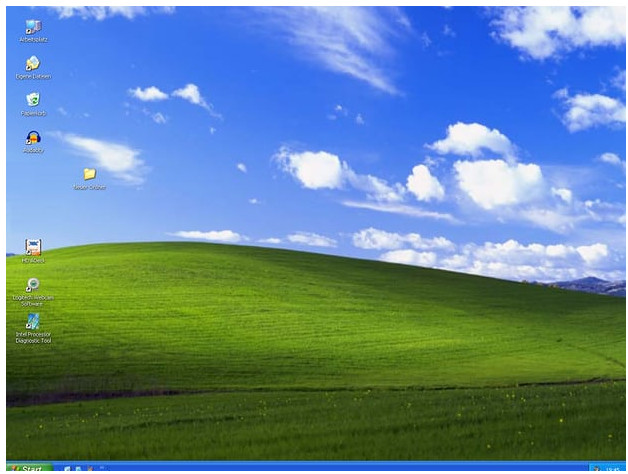
\includegraphics[scale=0.5]{wxp.jpg}
		\end{frame}
		\begin{frame}{Historia de Windows}
			Windows Vista fue lanzado en 2005. Hubo grandes modificaciones con respecto a XP:
			\begin{itemize}
				\item Seguridad mejorada
				\item Gráficas mejoradas
				\item Una mejor arquitectura para el sistema de archivos
				\item Reconocimiento de voz
				\item Windows Media Player 11, IE 7, Utilerias de restauración.
				\item Folder virtual
				\item Windows Aero
				\item Windows Automatic Updates
			\end{itemize}
		\end{frame}
		\begin{frame}{Historia de Windows}
			Una imagen de como era Windows vista
			
			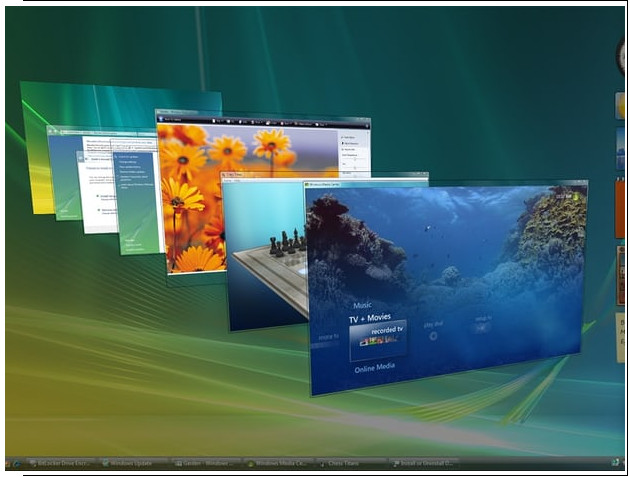
\includegraphics[scale=0.5]{wvista.jpg}
		\end{frame}		
		\begin{frame}{Historia de Windows}
			Windows 7 fue lanzado en octubre de 2009. Este sistema operativo sería el sucesor de la generaciñón XP. Tuvo ediciones de negocios, casera y de escritorio. Se mejoraron los gráficos, introduciendo los gráficos en 3D. Esta versión fue enfocada en ser \textit{users friendly}. 
			
			Una nueva arquitectura de la barra de tareas fue hecha. Igualmente se actualizaron los programas multimedia (Windows Movie Maker, Windows Media Player, etc.)
		\end{frame}
		\begin{frame}{Historia de Windows}
			Una imagen de como es Windows 7
			
			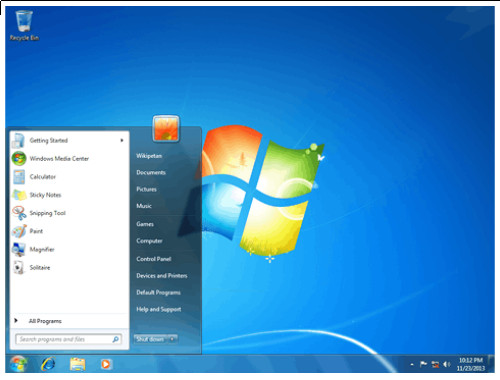
\includegraphics[scale=0.68]{w7.jpg}
		\end{frame}
\section{UNIX}
	\subsection{Qué es UNIX?}
		\begin{frame}{Qué es UNIX?}
			La marca UNIX ha sido aplicado a la familia de sistemas operativos de computadora que son multitarea y multiusuario que son derivados del sistema operativo original AT\& T UNIX desarrollado en los años 1970s en los laboratios Bell por Ken Thompson, Dennis Ritchie y demás.
			
			UNIX fue creado con la idea de diseñar un pequeño pero eficiente sistema operativo con una interfaz limpia. La filosofia de UNIX es: \textit{escribir programas que hagan una cosa y que la hagan bien. Escribir programas que trabajen juntos. Escribir programas que manejen los flujos de texto, porque esta es la interfaz universal.}
		\end{frame}
		\begin{frame}{Filosofia de UNIX}
			Toda la filosofia detras de UNIX se puede resumir en el principio KISS.
			
			
\includegraphics[scale=0.4]{unixfil.jpg}
		\end{frame}
	\subsection{Historia de UNIX}
		\begin{frame}{Historia de UNIX: 1969-1995}
			El UNIX original fue el tercer sistema de una serie de intentos.
			\begin{itemize}
				\item El primer intento fue el pequeño y simple \textit{Compatile Time-Sharing System} (CTSS), uno de los primeros sistemas desarrollados de tiempo compartido.
				\item El segundo intento fue el proyecto Multics, el cual fue un intento de crear un paquete de utilerias de la información que podria soportar tiempo compartido interactivo. El proyecto colapsó por su propio peso, pero de este colapso, nació UNIX.
			\end{itemize}
		\end{frame}
		\begin{frame}{Genesis: 1969-1971}
		 	\begin{itemize}
				\item Unix nació en 1969 de la menta de Ken Thompson en los laboratios Bell. Thompson había sido investigador en el proyecto Multics.
				\item Thompson tuvo ideas inspiradas en el proyecto Multics sobre como construir un sistema de archivos.
				
				\item Unix comenzó a cobrar vida en una minicomputadora PDP-7 como una plataforma para el juego Space Travel y como una plataforma de prueba para las ideas de Thompson sobre el diseño de un SO
				\item La PDP-7 tenía menos RAM y almacenamiento que un celular. En aquellos días un disco grande tenia menos de un megabyte de espacio.
		 	\end{itemize}
		\end{frame}
		\begin{frame}{Genesis: 1969-1971}
		 	\begin{itemize}
				\item Dennis Ritchie fue el primer colaborador de Thompson. Ritchie es conocido como co inventor de Unix e invetor del lenguaje C. Ritchie, McIlroy y algunos colegas que trabajaron en el proyecto Multics encontraron en el SO de Thompson una segunda oportunidad.
				\item Thompson y Ritchie escribiendo programas para dar soporte a el juego que se desarrollaba (Sapce Travel). Estos se convertirían en el núcleo de UNIX
				
				\item El nombre original fue UNICS (UNiplexed Information and Computing Service) el cual recordaba mucho a Multics (MULTIiplexed Information and Computing Service)
		 	\end{itemize}
		\end{frame}
		\begin{frame}{Genesis: 1969-1971}
			\begin{itemize}
				\item Las primeras versiones se nota un gran parecido a lo que es UNIX hoy.
				\item UNIX estuvo muy cerca de ser el primer sistema bajo el cual un programador podia sentarse en la maquina y hacer programas de inmediato.
				\item UNIX ha seguido un creciendo atrayendo a voluntarios altamente calificados para sobrepasar las limitaciones de otros SO.
				\item A diferencia de Multics, el cual era un gran proyecto y tenia miles de páginas de especificaciones técnicas, UNIX fue ideado por tres personas e implementado por Thompson en dos días
				\item En 1971, UNIX soportaba el procesador de textos para los Laboratorios Bell. Esto permitió que UNIX se estableciera como una parte permanente y valuada para la computación en Bell Labs
			\end{itemize}
		\end{frame}
		\begin{frame}{Éxodo: 1971-1980}
			\begin{itemize}
				\item En un inicio, UNIX estaba escrito en una mezcla de ensamblador y un lenguaje interpretado llamado B. Dennies Ritchie mejoró B resultando en el lenguaje C. En 1973 Thompson y Ritchie reescribieron UNIX en C.
				\item En 1974 Se realizó la primera exposición al público de UNIX. Diversos laboratorios de investigación y universidades alrededor del mundo pidieron una copia de UNIX.
				\item En esos años, las computadoras que podían correr UNIX solo podían adquirirlas grandes organizaciones como: corporaciones, universidades y agencias del gobierno.
				\item A lo largo de los años 70s, diversos grupos modificaban el interprete de comandos de UNIX, hacian mejoras en su rendimiento y producian versiones para más usuarios.
				\item Microsoft entraba a escena con sus productos como competencia a UNIX.
			\end{itemize}
		\end{frame}
		\begin{frame}{TCP/IP y la guerra de UNIX: 1980-1990}
			\begin{itemize}
				\item El campus de Berkeley de la universidad de California se convirtió en un importante punto de desarrollo académico de UNIX. En 1977 Se lanzó el primer Berkeley Software Release por un alumno: Bill Joy. Muchas ideas del UNIX de Berkeley fueron tomadas por Bell Labs (como Vi).
				\item En 1980, la Defense Advanced Research Projects Agency (DARPA) escogió a Berkeley UNIX como plataforma para implementar el protocolo TCP/IP (Comunicaciones de redes). Antes de esto, UNIX tenia un soporte débil en redes, por no decir un servicio de red horrible.
				\item La implementación de TCP/IP trajo consigo la combinación de Unix y ARPANET (red de computadoras creada para utilizarla como medio de comunicación entre las diferentes instituciones académicas y estatales.
			\end{itemize}
		\end{frame}
		\begin{frame}{TCP/IP y la guerra de UNIX: 1980-1990}
			\begin{itemize}
				\item En 1981, Microsoft se alió con IBM, lo que provocó que en la siguiente década, Bill Gates se hiciera multibillonario con código que no escribió (además de estrategías de negocios). Creo el monopolio en las computadoras de escritorio.
				\item Las computadoras de IBM no podían correr UNIX dado que no tenían el hardware suficiente. 1982 se lanzó Sun Microsystems y C se estableció, finalmente, como un lenguaje de programación independiente de UNIX.
				\item Sun Microsystems construiría maquinas de ensueño para correr UNIX. Combinarían el hardware diseñado en Standford y el UNIX de Berkeley. Lentamente UNIX dejo de ser código abierto.
			\end{itemize}
		\end{frame}
		\begin{frame}{TCP/IP y la guerra de UNIX: 1980-1990}
			\begin{itemize}
				\item Lentamente las estaciones de trabajo de Sun fueron tomando posición como las máquinas dominantes en internet.
				\item En 1983, por una movida gubernamental (contra Bell Labs), AT\&T paso a convertir a UNIX en un producto. Comercializó UNIX System V (lo que permitió que UNIX fuera conocido internacionalmente)
				\item Esta producción de UNIX destruiría los intercambios gratis de código que había contribuido a la vitalidad del SO. AT\&T detuvo las distribuciones de código y por lo tanto las contribuciones de las universidades se detuvieron.
			\end{itemize}
		\end{frame}
		\begin{frame}{TCP/IP y la guerra de UNIX: 1980-1990}
			\begin{itemize}
				\item Para poner peor las cosas, se propuso tomar ventaja de los diferentes productos, esto resulto en que las diferentes interfaces de UNIX divergieran, lo que destruyó la compatibilidad multiplataforma y la fragmentación de UNIX.
				\item Por otra parte, UNIX no tomo importancia a las computadoras personales, y las que tomaron en cuenta fueron aquellas para desarrolladores e ingenieros. Es por esto que Microsoft gano terreno en este campo.
				\item La guerra de UNIX (primera fase) consistió en una disputa entre el UNIX System V (Sun) y BSD UNIX (Berkeley). Esta disputa fuera tanto técnica como cultural. Existían programadores y técnicos que se decantaban por BSD y personas de negocios que preferían a AT\&T y UNIX V.
			\end{itemize}
		\end{frame}
		\begin{frame}{TCP/IP y la guerra de UNIX: 1980-1990}
			\begin{itemize}
				\item Larry Wall invento la herramienta de parches, originalmente era una herramienta que aplicaba ciertos cambios al archivo base. Esto permitió pasar una gran cantidad de código que actualizaba al anterior.
				\item En 1985, Intel lanzó uno de sus primeros chip. También, Richard Stallman lanzó la iniciativa GNU. Y se inició la máquina gráfica de UNIX.
				\item En 1986, Larry Wall empezo a trabajar en Perl, el cual fue el primer, y más usado, lenguaje de \textit{scripting} de código abierto.
				\item En 1987 apareció la versión GNU del compilador de C. Con el desarrollo del proyecto GNU, la gente entendió el daño que provocó la \textit{industrialización} a UNIX y a la comunidad.
			\end{itemize}
		\end{frame}
		\begin{frame}{TCP/IP y la guerra de UNIX: 1980-1990}
			\begin{itemize}
				\item La segunda fase de la guerra de UNIX empezó cuando vendedores como IBM, DEC, HP y otros, formaron la fundación de Software abierto contra el eje de AT\&T/Sun.
				\item Mientras Microsoft hacia billones en los mercados caseros y de pequeñas empresas. Con la salida de Windows 3.0, Microsoft marcó su dominio absoluto.
				\item Entre 1989 y 1993 Unix tuvo su más oscuras épocas: No podían competir contra Microsoft, los chip que eran preferidos por los programadores de UNIX (Motorola) fueron vencidos por Intel. El proyecto GNU falló en producir un kernel gratis de UNIX. Unix seguía siendo caro, a pesar de que el hardware bajo de precio.
			\end{itemize}
		\end{frame}
		\begin{frame}{Vientos contra el imperio: 1991-1995}
			\begin{itemize}
				\item En agosto de 1991, Linus Torvalds anuncio el projecto Linux. Torvals estaba motivado por el alto costo del Unix de Sun en su universidad.
				\item Linux se tornó de gran importancia para el mundo Unix con la explosión de internet de 1993-1994.
				\item El desarrollo de Linux y BSD se centro en los esfuerzos de los usuarios de internet. De esta manera, Linux se hizo de una interfaz de usuario gráfica.
				\item Linux siguió creciendo dado que era un sistema UNIX barato con la ayuda de internet. Mientras tanto, AT\&T perdió interés y vendió Unix Systems Laboratories a Novell. De aquí paso entre varias empresas hasta que el código base original de UNIX se vendo a Caldera, el cual era un distribuidor de Linux. 
			\end{itemize}
		\end{frame}
		\begin{frame}{Linux y el mocimiento Open-Source: de 1998 en adelante}
			\begin{itemize}
				\item Para estos años, el movimiento Open-Source cobró demasiada fuerza. La comunidad de Linux empezó a crecer de manera rápida al absorber a ciertos grupos de la internet.
				\item La cultura hacker empezó a empujar a Linux y el modelo de desarrollo tan lejos como se pudiera ir.
				\item Los hackers que vivieron en la era de Unix y presenciaron las \textit{guerras civiles} de los años 80s decidieron apoyar Linux como su último esfuerzo de cumplir sus sueños de los primeros días de Unix.	
				\item El movimiento Open Source se consolidó como ideológicamente neutro, tratando de hacer frente al monopolio de Microsoft de manera pasiva. 		
			\end{itemize}
		\end{frame}
	\subsection{Unix en el presente}
		\begin{frame}{Características de Unix}
			\begin{itemize}
				\item Una de las ideas más importantes de Unix es el modelo: todo es un archivo y la metáfora de \textit{tuberias}. Por esto, Unix se vasa en la idea de unificar ideas.
				\item Unix se basa en la multitarea con preferencias. Esto quiere decir que se puede interrumpir otro proceso por correr un proceso más importante. En la actualidad, casi todos los SO hacen esto.
				\item Unix está hecho suponiendo que el programador sabe que es lo mejor. A pesar de esto, se esfuerza por que la información de un usuario no pueda ser tocada por otros usuarios. Por lo que tiene fronteras internas muy bien definidas.
			\end{itemize}
		\end{frame}
		\begin{frame}{Características de Unix}
			\begin{itemize}
				\item En Unix los archivos no tienen ni estructura de registro ni atributos a diferencia de otros SO como Windows.
				\item Unix generalmente no maneja archivos en formato binario. Dado que se requiere de herramientas pesadas para leerlos y editarlos. Además de que estos no pueden ser leídos fácilmente.
				\item En Unix se prefiere la interface por línea de comandos que una interfaz gráfica.
				\item En Unix no existirán barreras para que se experimente en la programación.
			\end{itemize}
		\end{frame}
		\begin{frame}{Qué es MacOs?}
			\begin{itemize}
				\item MasOs ha tomado ideas de la infraestructura de Unix. A pesar de que sigue fuertemente las versiones de Unix, este se enfoca fuertemente en la interfaz.
				\item A pesar de que las facilidades para programar están presentes comúnmente no son usadas como en Unix. 
				\item El diseño del SO se enfoca en tener una separación, relativamente limpia, entre la aplicación y la interfaz gráfica.
				\item MacOs está diseñado para que los usuarios finales no tengan que saber cosas técnicas, por lo que la complejidad de la interfaz es mínima.
			\end{itemize}
		\end{frame}
		\begin{frame}{Qué es Linux?}
			\begin{itemize}
				\item Linux dirige la nueva escuela del código abierto de Unixs que emergieron desde 1990. La dirección de diseño es decidida en grupo.
				\item Linux no incluye ningún código del Unix original, pero esta diseñado de los estándares de Unix lo que lo hace ser un Unix. Hay una continuidad entre Unix y Linux en términos de tecnología y desarrollo.
				\item A diferencia del Unix original, Linux y sus desarrolladores pretenden compartir una gran cantidad de usuarios finales en equipos de escritorio. 
			\end{itemize}
		\end{frame}
		\begin{frame}{Qué es Linux?}
			\begin{itemize}
				\item El cambio más importante fue cambiar el estilo de la interfaz. Unix estaba diseñado originalmente para usar terminales y a lo largo de su vida fue asociado a esto a pesar de que se han desarrollado interfaces gráficas.
				\item Linux aún no ha perdido esta idea, pero han desarrollado muchas herramientas gráficas que ayudan a los nuevos usuarios a moverse de una plataforma a otra.
				\item Además, Linux y su comunidad se ha expandido para conectarse con otros ambientes. Es decir, tiene soporte para escribir en otros sistemas de archivos y comunicación de red con otros SO. Además de permitir convivir en una misma máquina con otros SOs.
			\end{itemize}
			%\pause
			%Vamos a aprender Linux!!
		\end{frame}
\end{document}